% !TEX program = xelatex
% ============================================================================
%  POSN Computer Qualification — 3D Shapes
%  Topic: รูปสามมิติ (3D Shapes)
% ============================================================================

\documentclass[11pt, aspectratio=169]{beamer}
% ============================================================================
%  POSN Computer Qualification — Shared Beamer Preamble
%  Used by all topic slide decks. Compile with XeLaTeX.
% ============================================================================

% ---------- Thai language & font ----------
\usepackage{iftex}
\usepackage{fontspec}

% XeTeX-specific: enable Thai line breaking
\ifXeTeX
  \XeTeXlinebreaklocale{th}
\fi
% Noto Sans Thai — body text (clean modern sans-serif, handles all Thai)
\setmainfont{Noto Sans Thai}[
  UprightFont = Noto Sans Thai Light,
  BoldFont    = Noto Sans Thai Medium,
  Scale       = 0.9
]
\setsansfont{Noto Sans Thai}[
  UprightFont = Noto Sans Thai Light,
  BoldFont    = Noto Sans Thai Medium,
  Scale       = 0.9
]

% Noto Sans Thai — clean modern sans-serif for structural elements
\newfontfamily\headingfont{Noto Sans Thai}[
  UprightFont = Noto Sans Thai Medium,
  BoldFont    = Noto Sans Thai Bold,
  Scale       = 0.9
]

% --- Heading font for structural elements ---
\setbeamerfont{title}{family=\headingfont, series=\bfseries, size=\huge}
\setbeamerfont{subtitle}{family=\headingfont, series=\mdseries}
\setbeamerfont{author}{family=\headingfont, series=\mdseries}

% --- Custom Title Page ---
\defbeamertemplate{title page}{custom}[1][]{%
  \centering
  \vspace*{2cm}
  % Title — in white
  {\usebeamerfont{title}\color{white}\inserttitle\par}
  \vspace{0.6cm}
  % Subtitle — in white
  {\usebeamerfont{subtitle}\color{white}\insertsubtitle\par}
  \vspace{2.5cm}
  % Author — blue filled rounded box, white text
  \begin{center}
    \begin{tcolorbox}[arc=3mm, colback=boxBlue, colframe=boxBlue!80,
                      width=0.42\textwidth, halign=center,
                      left=1.5em, right=1.5em, top=0.8em, bottom=0.8em,
                      boxrule=1.5pt, coltext=white]
      \usebeamerfont{author}\insertauthor
    \end{tcolorbox}
  \end{center}
}
\setbeamertemplate{title page}[custom]
\setbeamerfont{frametitle}{family=\headingfont, series=\bfseries}
\setbeamerfont{section in toc}{family=\headingfont}
\setbeamerfont{page number in head/foot}{family=\headingfont}
\setbeamerfont{section title}{family=\headingfont, series=\bfseries}
\setbeamerfont{subsection title}{family=\headingfont}

% Monospace font (for code/verbatim)
\setmonofont{Latin Modern Mono}[Scale=0.9]

% ---------- Math ----------
\usepackage{amsmath, amssymb}

% ---------- Graphics ----------
\usepackage{graphicx}
\usepackage{tikz}

% ---------- String parsing (for section headers) ----------
\usepackage{xstring}

% ---------- Colored boxes ----------
\usepackage[skins, breakable, xparse]{tcolorbox}
% Note: we do NOT load the 'most' option — it predefines example/solution environments
% that would conflict with our custom boxes.

% --- Color definitions ---
\definecolor{boxBlue}{RGB}{41, 128, 185}
\definecolor{boxGreen}{RGB}{39, 174, 96}
\definecolor{boxOrange}{RGB}{230, 126, 34}
\definecolor{boxPurple}{RGB}{142, 68, 173}
\definecolor{boxBlueBg}{RGB}{235, 245, 255}
\definecolor{boxGreenBg}{RGB}{235, 255, 240}
\definecolor{boxOrangeBg}{RGB}{255, 245, 235}
\definecolor{boxPurpleBg}{RGB}{248, 240, 255}

% --- Explanation box (blue) — for definitions, concepts, notes ---
\newtcolorbox{explanation}[1][]{
  enhanced,
  breakable,
  arc         = 2mm,
  colback     = boxBlueBg,
  colframe    = boxBlue!50,
  title       = #1,
  fonttitle   = \bfseries\color{white},
  coltitle    = white,
  colbacktitle= boxBlue,
  attach boxed title to top left = {yshift=-2mm, xshift=2mm},
  boxed title style = {arc=2mm, size=small},
  before skip = 8pt,
  after skip  = 8pt
}

% --- Example box (green) — for worked examples ---
\newtcolorbox{exambox}[1][]{
  enhanced,
  breakable,
  arc         = 2mm,
  colback     = boxGreenBg,
  colframe    = boxGreen!50,
  title       = #1,
  fonttitle   = \bfseries\color{white},
  coltitle    = white,
  colbacktitle= boxGreen,
  attach boxed title to top left = {yshift=-2mm, xshift=2mm},
  boxed title style = {arc=2mm, size=small},
  before skip = 8pt,
  after skip  = 8pt
}

% --- Solution box (orange) — for solutions and answers ---
\newtcolorbox{solbox}[1][]{
  enhanced,
  breakable,
  arc         = 2mm,
  colback     = boxOrangeBg,
  colframe    = boxOrange!50,
  title       = #1,
  fonttitle   = \bfseries\color{white},
  coltitle    = white,
  colbacktitle= boxOrange,
  attach boxed title to top left = {yshift=-2mm, xshift=2mm},
  boxed title style = {arc=2mm, size=small},
  before skip = 8pt,
  after skip  = 8pt
}

% --- Intuition box (purple) — for plain-language explanations, analogies ---
\newtcolorbox{intuition}[1][]{
  enhanced,
  breakable,
  arc         = 2mm,
  colback     = boxPurpleBg,
  colframe    = boxPurple!50,
  title       = #1,
  fonttitle   = \bfseries\color{white},
  coltitle    = white,
  colbacktitle= boxPurple,
  attach boxed title to top left = {yshift=-2mm, xshift=2mm},
  boxed title style = {arc=2mm, size=small},
  before skip = 8pt,
  after skip  = 8pt
}

% ---------- Beamer theme ----------
\usetheme{Madrid}
\usecolortheme{default}

% --- Custom beamer colors (blue accent matching explanation boxes) ---
\setbeamercolor{structure}{fg=boxBlue}
\setbeamercolor{palette primary}{fg=white, bg=boxBlue}
\setbeamercolor{palette secondary}{fg=white, bg=boxBlue!80}
\setbeamercolor{palette tertiary}{fg=white, bg=boxBlue!60}
\setbeamercolor{block title}{fg=white, bg=boxBlue}
\setbeamercolor{block body}{fg=black, bg=boxBlueBg}

% Remove navigation symbols for clean look
\setbeamertemplate{navigation symbols}{}

% Note: Frame title prefix removed — \addtobeamertemplate conflicts with beamer internals

% --- Outline (Table of Contents) styling ---
\setbeamerfont{section in toc}{family=\headingfont, series=\mdseries}
\setbeamerfont{subsection in toc}{family=\headingfont, series=\mdseries}
\setbeamertemplate{section in toc}{%
  \leavevmode\leftskip=1.5em
  \textcolor{boxBlue}{\textbf{\large\inserttocsectionnumber.}}%
  \quad\inserttocsection\par
  \vspace{0.2em}
}
\setbeamertemplate{subsection in toc}{%
  \leavevmode\leftskip=4em
  \textcolor{boxBlue!60}{\small$\bullet$}%
  \quad\inserttocsubsection\par
  \vspace{0.1em}
}

% Section header slides — Thai in white, English in smaller light blue below
\AtBeginSection{
  \begin{frame}[plain]{}
    \vspace*{2cm}
    \begin{beamercolorbox}[sep=12pt, center, rounded=true, shadow=true]{palette primary}
      \IfSubStr{\secname}{(}{%
        \StrBefore{\secname}{(}[\sectionthai]%
        \StrBetween[1,1]{\secname}{(}{)}[\sectioneng]%
        \begin{tabular}{@{}c@{}}
          {\usebeamerfont{title}\sectionthai} \\[0.2em]
          {\usebeamerfont{subtitle}\color{boxBlue!60}\sectioneng}
        \end{tabular}%
      }{%
        {\usebeamerfont{title}\secname\par}%
      }
    \end{beamercolorbox}
    \vfill
  \end{frame}
}

% Subsection header slides — smaller, centered
\AtBeginSubsection{
  \begin{frame}[plain]{}
    \vfill
    \centering
    {\usebeamerfont{section title}\insertsubsectionhead\par}
    \vfill
  \end{frame}
}

% Minimal footer: page number only, right-aligned
\setbeamertemplate{footline}{
  \hfill\usebeamerfont{page number in head/foot}\insertframenumber{} / \inserttotalframenumber\hspace*{1em}\vspace*{0.5ex}
}

% ---------- Spacing & readability ----------
\linespread{1.2}

% ---------- Useful commands ----------

% Highlight important text in blue
\newcommand{\highlight}[1]{\textcolor{boxBlue}{\textbf{#1}}}

% Math set notation helpers
\newcommand{\R}{\mathbb{R}}
\newcommand{\N}{\mathbb{N}}
\newcommand{\Z}{\mathbb{Z}}
\newcommand{\Q}{\mathbb{Q}}

% ============================================================================
%  End of preamble
% ============================================================================


\title[รูปสามมิติ]{\textcolor{white}{รูปสามมิติ} \textcolor{boxBlue!60}{(3D Shapes)}}
\subtitle{ปริซึม • พีระมิด • ทรงกระบอก • กรวย • ทรงกลม • ปริมาตร • พื้นที่ผิว }
\author[None W. (Yuan)]{None W. (Yuan)}
\date{}

\begin{document}

\begin{frame}[plain]\titlepage\end{frame}
\begin{frame}{สารบัญ (Outline)}\tableofcontents\end{frame}

\begin{frame}{ก่อนเรียน (Prerequisites)}
  \begin{explanation}[สิ่งที่ควรรู้ก่อนเรียน]
    \begin{itemize}
      \item \textbf{รูปสองมิติ} — พื้นที่สามเหลี่ยม, สี่เหลี่ยม, วงกลม, เส้นรอบรูป
      \item \textbf{ทฤษฎีบทพีทาโกรัส} — $c^2 = a^2 + b^2$
      \item \textbf{เลขยกกำลัง} — $x^2$, $x^3$, $\sqrt{x}$
      \item \textbf{สมการ} — การแก้สมการเชิงเส้น
    \end{itemize}
  \end{explanation}

  \begin{intuition}[รูปสามมิติคืออะไร?]
    \textbf{รูปสามมิติ} คือรูปเรขาคณิตที่มี \textbf{ความกว้าง ความยาว และความสูง}
    — มี \textbf{ปริมาตร} (ความจุ) และ \textbf{พื้นที่ผิว} (พื้นที่ทั้งหมดของผิวภายนอก)
  \end{intuition}
\end{frame}

% ===========================================================================
%  SECTION 1: รู้จักรูปสามมิติ
% ===========================================================================
\section{รู้จักรูปสามมิติ (Introduction)}

\begin{frame}{หน้าตัด จุดยอด และขอบ (Faces, Vertices, Edges)}
  \begin{explanation}[ส่วนประกอบของทรงหลายหน้า (Polyhedron)]
    \begin{itemize}
      \item \textbf{หน้า (Face)} — ระนาบแต่ละด้านของรูป
      \item \textbf{ขอบ (Edge)} — เส้นที่เกิดจากหน้าสองหน้ามาบรรจบกัน
      \item \textbf{จุดยอด (Vertex)} — จุดที่ขอบมาบรรจบกัน
    \end{itemize}
  \end{explanation}

  \begin{columns}[T]
    \column{0.45\textwidth}
      \centering
      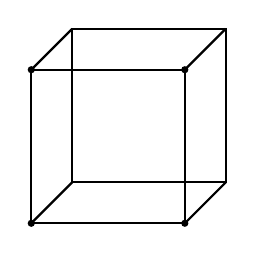
\begin{tikzpicture}[scale=1.3]
        % Simple cube
        \draw[thick] (0,0) -- (1.5,0) -- (1.5,1.5) -- (0,1.5) -- cycle;
        \draw[thick] (0.4,0.4) -- (1.9,0.4) -- (1.9,1.9) -- (0.4,1.9) -- cycle;
        \draw[thick] (0,0) -- (0.4,0.4);
        \draw[thick] (1.5,0) -- (1.9,0.4);
        \draw[thick] (1.5,1.5) -- (1.9,1.9);
        \draw[thick] (0,1.5) -- (0.4,1.9);
        \foreach \p in {(0,0),(0,1.5),(1.5,1.5),(1.5,0)}
          \fill \p circle (1pt);
      \end{tikzpicture}

      \textbf{ทรงหลายหน้า (Polyhedron)}

      หน้าทั้งหมดเป็นรูปหลายเหลี่ยม

    \column{0.55\textwidth}
      \begin{exambox}[สูตรของออยเลอร์ (Euler's Formula)]
        สำหรับทรงหลายหน้านูน:
         $F + V - E = 2$
        \begin{itemize}
          \item ลูกบาศก์: $6 + 8 - 12 = 2$ \quad $\checkmark$
          \item พีระมิดฐานสี่เหลี่ยม: $5 + 5 - 8 = 2$ \quad $\checkmark$
        \end{itemize}
      \end{exambox}
  \end{columns}
\end{frame}

\begin{frame}{ทรงหลายหน้ากับรูปทรงผิวโค้ง}
  \begin{columns}[T]
    \column{0.5\textwidth}
      \centering
      \textbf{ทรงหลายหน้า (Polyhedron)}

      \medskip
      \begin{tikzpicture}[scale=1.1]
        % Triangular prism — oblique projection, shift=(0.4,0.5)
        % Front triangle
        \draw[thick] (0,0) -- (1.5,0) -- (0.75,1.3) -- cycle;
        % Back triangle (shifted by 0.4,0.5)
        \draw[thick] (0.4,0.5) -- (1.9,0.5) -- (1.15,1.8) -- cycle;
        % Connecting edges: all parallel to shift vector
        \draw[thick] (0,0) -- (0.4,0.5);
        \draw[thick] (1.5,0) -- (1.9,0.5);
        \draw[thick] (0.75,1.3) -- (1.15,1.8);
        \node at (1.0,-0.5) {ปริซึมสามเหลี่ยม};
      \end{tikzpicture}

      \begin{itemize}
        \item ทุกหน้าเป็นรูปหลายเหลี่ยม
        \item ปริซึม, พีระมิด, ลูกบาศก์
      \end{itemize}

    \column{0.5\textwidth}
      \centering
      \textbf{รูปทรงผิวโค้ง (Non-Polyhedron)}

      \medskip
      \begin{tikzpicture}[scale=1.1]
        % Cylinder
        \draw[thick] (0,0) ellipse (1.2 and 0.4);
        \draw[thick] (0,2) ellipse (1.2 and 0.4);
        \draw[thick] (-1.2,0) -- (-1.2,2);
        \draw[thick] (1.2,0) -- (1.2,2);
        \node at (0,-0.7) {ทรงกระบอก};
      \end{tikzpicture}

      \begin{itemize}
        \item มีผิวโค้ง (curved surface)
        \item ทรงกระบอก, กรวย, ทรงกลม
      \end{itemize}
  \end{columns}
\end{frame}

% ===========================================================================
%  SECTION 2: ปริซึม
% ===========================================================================
\section{ปริซึม (Prism)}

\begin{frame}{ปริซึมคืออะไร?}
  \begin{explanation}[นิยาม]
    \textbf{ปริซึม} คือทรงหลายหน้าที่มี \highlight{หน้าตัดสองหน้าเท่ากันทุกประการและขนานกัน}
    หน้าข้างทุกหน้าเป็นสี่เหลี่ยมด้านขนาน
  \end{explanation}

  \begin{columns}[T]
    \column{0.33\textwidth}
      \medskip\medskip\medskip\medskip
      \centering
      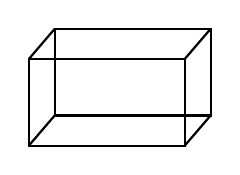
\begin{tikzpicture}[scale=1.1]
        % Rectangular prism (cuboid)
        \draw[thick] (0,0) -- (1.8,0) -- (1.8,1) -- (0,1) -- cycle;
        \draw[thick] (0.3,0.35) -- (2.1,0.35) -- (2.1,1.35) -- (0.3,1.35) -- cycle;
        \draw[thick] (0,0) -- (0.3,0.35);
        \draw[thick] (1.8,0) -- (2.1,0.35);
        \draw[thick] (1.8,1) -- (2.1,1.35);
        \draw[thick] (0,1) -- (0.3,1.35);
      \end{tikzpicture}
      \textbf{ปริซึมสี่เหลี่ยม}

    \column{0.33\textwidth}
      \centering
      \medskip\medskip\medskip\medskip
      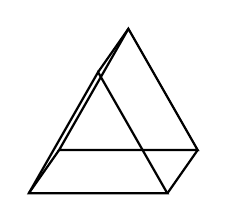
\begin{tikzpicture}[scale=1.1]
        % Triangular prism — oblique shift (0.35, 0.5)
        % Front triangle
        \draw[thick] (0,0) -- (1.6,0) -- (0.8,1.4) -- cycle;
        % Back triangle = front shifted by (0.35, 0.5)
        \draw[thick] (0.35,0.5) -- (1.95,0.5) -- (1.15,1.9) -- cycle;
        % Connecting edges (all parallel to shift vector)
        \draw[thick] (0,0)   -- (0.35,0.5);
        \draw[thick] (1.6,0) -- (1.95,0.5);
        \draw[thick] (0.8,1.4) -- (1.15,1.9);
      \end{tikzpicture}
      \textbf{ปริซึมสามเหลี่ยม}

    \column{0.33\textwidth}
      \centering
      \medskip\medskip\medskip\medskip
      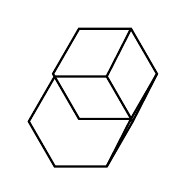
\begin{tikzpicture}[scale=1.1]
        % Regular hexagon prism — oblique shift (0.28, 0.55)
        % Front regular hexagon (center ~(0.7, 0.7), radius 0.6)
        \draw[thick] (1.3,0.7) -- (1.0,1.22) -- (0.4,1.22) -- (0.1,0.7) --
                     (0.4,0.18) -- (1.0,0.18) -- cycle;
        % Back hexagon (shifted)
        \draw[thick] (1.58,1.25) -- (1.28,1.77) -- (0.68,1.77) -- (0.38,1.25) --
                     (0.68,0.73) -- (1.28,0.73) -- cycle;
        % Visible edges (front-right side)
        \draw[thick] (1.3,0.7) -- (1.58,1.25);
        \draw[thick] (1.0,1.22) -- (1.28,1.77);
        \draw[thick] (1.0,0.18) -- (1.28,0.73);
      \end{tikzpicture}
      \textbf{ปริซึมหกเหลี่ยม}
  \end{columns}
\end{frame}

\begin{frame}{ปริมาตรและพื้นที่ผิวของปริซึม}
  \begin{explanation}[สูตร]
    \begin{itemize}
      \item \textbf{ปริมาตร} $V =$ \highlight{พื้นที่ฐาน $\times$ ความสูง} $= A_{\text{base}} \times h$
      \item \textbf{พื้นที่ผิว} $= 2 \times$ พื้นที่ฐาน $+$ พื้นที่ผิวข้าง
      \item \textbf{พื้นที่ผิวข้าง} $=$ เส้นรอบรูปฐาน $\times$ ความสูง
    \end{itemize}
  \end{explanation}

  \begin{columns}[T]
    \column{0.5\textwidth}
      \centering
      \medskip\medskip\medskip\medskip
      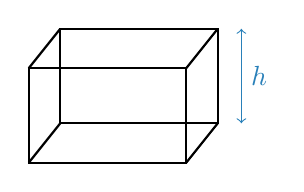
\begin{tikzpicture}[scale=1.0]
        \draw[thick] (0,0) -- (2,0) -- (2,1.2) -- (0,1.2) -- cycle;
        \draw[thick] (0.4,0.5) -- (2.4,0.5) -- (2.4,1.7) -- (0.4,1.7) -- cycle;
        \draw[thick] (0,0) -- (0.4,0.5);
        \draw[thick] (2,0) -- (2.4,0.5);
        \draw[thick] (2,1.2) -- (2.4,1.7);
        \draw[thick] (0,1.2) -- (0.4,1.7);
        \draw[boxBlue, <->] (2.7, 0.5) -- node[right] {$h$} (2.7,1.7);
      \end{tikzpicture}

    \column{0.5\textwidth}
      \begin{exambox}[ลูกบาศก์และทรงสี่เหลี่ยมมุมฉาก]
        \textbf{ลูกบาศก์} ด้าน $s$: $V = s^3$, $SA = 6s^2$

        \medskip
        \textbf{สี่เหลี่ยมมุมฉาก} $(\ell, w, h)$:
        $V = \ell w h$, $SA = 2(\ell w + \ell h + wh)$
      \end{exambox}
  \end{columns}
\end{frame}

\begin{frame}{ตัวอย่าง: ปริซึม}
  \begin{exambox}[โจทย์]
    ปริซึมฐานสามเหลี่ยมมุมฉาก มีด้านประกอบมุมฉากยาว 3 และ 4 ซม.
    ปริซึมสูง 10 ซม. จงหาปริมาตรและพื้นที่ผิว
  \end{exambox}

  \begin{solbox}[วิธีทำ]
    \textbf{พื้นที่ฐาน:} $A_{\text{base}} = \frac{1}{2} \times 3 \times 4 = 6$ ตร.ซม.

    \textbf{ปริมาตร:} $V = A_{\text{base}} \times h = 6 \times 10 = 60$ ลบ.ซม.

    \textbf{พื้นที่ผิว:} ด้านตรงข้ามมุมฉากของฐาน $= \sqrt{3^2 + 4^2} = 5$ ซม.
    \par เส้นรอบรูปฐาน $= 3 + 4 + 5 = 12$ ซม.
    \par พื้นที่ผิวข้าง $= 12 \times 10 = 120$ ตร.ซม.
    \par พื้นที่ผิวทั้งหมด $= 2(6) + 120 = 132$ ตร.ซม.
  \end{solbox}
\end{frame}

% ===========================================================================
%  SECTION 3: พีระมิด
% ===========================================================================
\section{พีระมิด (Pyramid)}

\begin{frame}{พีระมิดคืออะไร?}
  \begin{explanation}[นิยาม]
    \textbf{พีระมิด} คือทรงหลายหน้าที่มี \highlight{ฐานเป็นรูปหลายเหลี่ยม}
    และมี \highlight{หน้าข้างเป็นรูปสามเหลี่ยม} มาบรรจบกันที่ \textbf{จุดยอด} เดียว
  \end{explanation}

  \begin{columns}[T]
    \column{0.5\textwidth}
      \centering
      \medskip\medskip\medskip\medskip
      \begin{tikzpicture}[scale=1.2]
        % Square pyramid — base as oblique parallelogram
        % Base edges: front, right, back (hidden), left
        \draw[thick] (0,0) -- (1.8,0.3);                     % front
        \draw[thick] (1.8,0.3) -- (1.8,1.5);                 % right
        \draw[thick, dashed] (1.8,1.5) -- (0,1.8);           % back (hidden)
        \draw[thick] (0,1.8) -- (0,0);                       % left
        % Apex
        \fill (0.9,2.3) circle (1.2pt);
        \draw[thick] (0,0) -- (0.9,2.3);
        \draw[thick] (1.8,0.3) -- (0.9,2.3);
        \draw[thick] (1.8,1.5) -- (0.9,2.3);
        \draw[thick, dashed] (0,1.8) -- (0.9,2.3);           % back edge (hidden)
        \node at (0.9,-0.3) {พีระมิดฐานสี่เหลี่ยม};
      \end{tikzpicture}

    \column{0.5\textwidth}
      \centering
      \medskip\medskip\medskip\medskip
      \begin{tikzpicture}[scale=1.2]
        % Regular tetrahedron (clear base + apex above)
        % Base triangle (slightly tilted)
        \draw[thick] (0,0) -- (1.8,0.2) -- (0.9,1.5) -- cycle;
        \draw[thick, dashed] (0,0) -- (0.9,1.5);
        % Apex clearly above center
        \fill (0.85,2.2) circle (1.2pt);
        \draw[thick] (0,0) -- (0.85,2.2);
        \draw[thick] (1.8,0.2) -- (0.85,2.2);
        \draw[thick] (0.9,1.5) -- (0.85,2.2);
        \node at (0.9,-0.35) {ทรงสี่หน้า (Tetrahedron)};
      \end{tikzpicture}
  \end{columns}
\end{frame}

\begin{frame}{ปริมาตรและพื้นที่ผิวของพีระมิด}
  \begin{explanation}[สูตร]
    \begin{itemize}
      \item \textbf{ปริมาตร} $V = \frac{1}{3} \times$ \highlight{พื้นที่ฐาน $\times$ ความสูง} $= \frac{1}{3}A_{\text{base}}h$
      \item \textbf{พื้นที่ผิว} $=$ พื้นที่ฐาน $+$ ผลรวมพื้นที่หน้าสามเหลี่ยมทุกด้าน
    \end{itemize}
  \end{explanation}

  \begin{columns}[T]
    \column{0.3\textwidth}
      \centering
      \medskip\medskip\medskip\medskip
      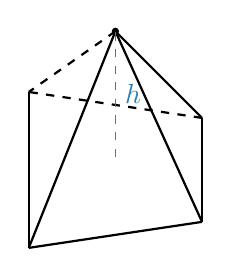
\begin{tikzpicture}[scale=1.1]
        \draw[thick] (0,0) -- (2,0.3);                     % front base edge
        \draw[thick] (2,0.3) -- (2,1.5);                   % right base edge
        \draw[thick, dashed] (2,1.5) -- (0,1.8);           % back base edge (hidden)
        \draw[thick] (0,1.8) -- (0,0);                     % left base edge
        \fill (1,2.5) circle (1.2pt);                      % apex
        \draw[thick] (1,2.5) -- (0,0);
        \draw[thick] (1,2.5) -- (2,0.3);
        \draw[thick] (1,2.5) -- (2,1.5);
        \draw[thick, dashed] (1,2.5) -- (0,1.8);           % back lateral edge (hidden)
        % Height line
        \draw[boxBlue, dashed] (1,1.05) -- (1,2.5) node[midway, right] {$h$};
      \end{tikzpicture}

    \column{0.7\textwidth}
      \begin{exambox}[ตัวอย่าง]
        พีระมิดฐานสี่เหลี่ยมจัตุรัสยาวด้านละ 6 ซม. สูง 4 ซม.

        $V = \frac{1}{3} \times 6^2 \times 4 = 48$ ลบ.ซม.
      \end{exambox}

      \begin{intuition}[ทำไมต้อง $\frac{1}{3}$?]
        พีระมิด 3 อันประกอบกันเป็นปริซึมพอดี! (เมื่อฐานเท่ากันและสูงเท่ากัน)
      \end{intuition}
  \end{columns}
\end{frame}

% ===========================================================================
%  SECTION 4: ทรงกระบอก
% ===========================================================================
\section{ทรงกระบอก (Cylinder)}

\begin{frame}{ทรงกระบอก}
  \begin{columns}[T]
    \column{0.4\textwidth}
      \centering
      \medskip\medskip\medskip\medskip\medskip\medskip
      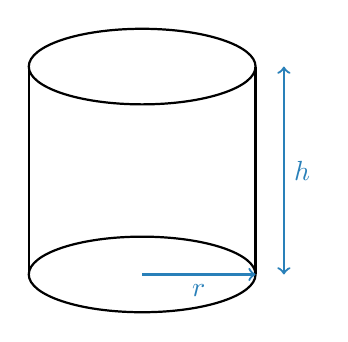
\begin{tikzpicture}[scale=1.2]
        \draw[thick] (0,0) ellipse (1.2 and 0.4);
        \draw[thick] (0,2.2) ellipse (1.2 and 0.4);
        \draw[thick] (-1.2,0) -- (-1.2,2.2);
        \draw[thick] (1.2,0) -- (1.2,2.2);
        \draw[boxBlue, thick, ->] (0,0) -- (1.2,0) node[midway, below] {$r$};
        \draw[boxBlue, thick, <->] (1.5,0) -- node[right] {$h$} (1.5,2.2);
      \end{tikzpicture}

    \column{0.61\textwidth}
      \begin{explanation}[สูตร]
        \begin{itemize}
          \item \textbf{ปริมาตร}: $V = \pi r^2 h$ \ (พื้นที่ฐาน $\times$ สูง)
          \item \textbf{พื้นที่ผิวข้าง}: $2\pi rh$ \ (เส้นรอบวง $\times$ สูง)
          \item \textbf{พื้นที่ผิวทั้งหมด}: $SA = 2\pi r^2 + 2\pi rh = 2\pi r(r+h)$
        \end{itemize}
      \end{explanation}

      \begin{exambox}[ตัวอย่าง]
        $r=7,\;h=10,\;\pi \approx \frac{22}{7}$:
        \\ $V = \frac{22}{7} \times 49 \times 10 = 1{,}540$ ลบ.ซม.
        \\ $SA = 2 \cdot \frac{22}{7} \cdot 7 \cdot 17 = 748$ ตร.ซม.
      \end{exambox}
  \end{columns}
\end{frame}

% ===========================================================================
%  SECTION 5: กรวย
% ===========================================================================
\section{กรวย (Cone)}

\begin{frame}{กรวย}
  \begin{columns}[T]
    \column{0.45\textwidth}
      \centering
      \medskip\medskip\medskip\medskip\medskip\medskip
      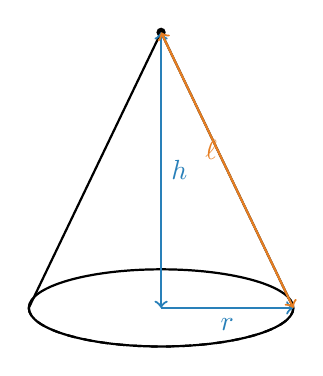
\begin{tikzpicture}[scale=1.4]
        % Cone
        \draw[thick] (0,0) ellipse (1.2 and 0.35);
        \draw[thick] (-1.2,0) -- (0,2.5);
        \draw[thick] (1.2,0) -- (0,2.5);
        \draw[thick, dashed] (-1.2,0) arc (180:360:1.2 and 0.35);
        \fill (0,2.5) circle (1.2pt);
        % Radius
        \draw[boxBlue, thick, ->] (0,0) -- (1.2,0) node[midway, below] {$r$};
        % Height
        \draw[boxBlue, thick, <->] (0,0) -- node[right] {$h$} (0,2.5);
        % Slant height
        \draw[boxOrange, thick, <->] (0,2.5) -- node[above left] {$\ell$} (1.2,0);
      \end{tikzpicture}

    \column{0.55\textwidth}
      \begin{explanation}[สูตร]
        \begin{itemize}
          \item \textbf{ปริมาตร}: $V = \frac{1}{3}\pi r^2 h$
          \item \textbf{สูงเอียง (slant height)}:
          \[
            \ell = \sqrt{r^2 + h^2}
          \]
          \item \textbf{พื้นที่ผิวข้าง}: $= \pi r \ell$
          \item \textbf{พื้นที่ผิวทั้งหมด}:
          \[
            SA = \pi r^2 + \pi r \ell = \pi r(r + \ell)
          \]
        \end{itemize}
      \end{explanation}
  \end{columns}
\end{frame}

\begin{frame}{ตัวอย่าง: กรวย}
  \begin{exambox}[โจทย์]
    กรวยมีรัศมีฐาน 6 ซม. สูง 8 ซม. จงหาปริมาตร, สูงเอียง และพื้นที่ผิวทั้งหมด
  \end{exambox}

  \begin{solbox}[วิธีทำ]
    \textbf{ปริมาตร:} $V = \frac{1}{3}\pi (6^2)(8) = \frac{1}{3}\pi (36)(8) = 96\pi$ ลบ.ซม.

    \textbf{สูงเอียง:} $\ell = \sqrt{6^2 + 8^2} = \sqrt{36+64} = \sqrt{100} = 10$ ซม.

    \textbf{พื้นที่ผิว:} $SA = \pi r^2 + \pi r \ell = 36\pi + 60\pi = 96\pi$ ตร.ซม.
  \end{solbox}

  \begin{intuition}[สังเกต!]
    ในตัวอย่างนี้ $V = 96\pi$ ลบ.ซม. และ $SA = 96\pi$ ตร.ซม. — ตัวเลขเท่ากันแต่หน่วยต่างกัน!
  \end{intuition}
\end{frame}

% ===========================================================================
%  SECTION 6: ทรงกลม
% ===========================================================================
\section{ทรงกลม (Sphere)}

\begin{frame}{ทรงกลม}
  \begin{columns}[T]
    \column{0.45\textwidth}
      \centering
      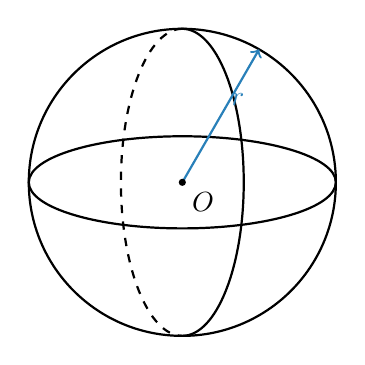
\begin{tikzpicture}[scale=1.3]
        \draw[thick] (0,0) circle (1.5);
        \draw[thick] (0,0) ellipse (1.5 and 0.45);
        \draw[thick] (0,1.5) arc (90:-90:0.6 and 1.5);
        \draw[thick, dashed] (0,1.5) arc (90:270:0.6 and 1.5);
        \draw[boxBlue, thick, ->] (0,0) -- (60:1.5) node[midway, above right] {$r$};
        \fill (0,0) circle (1pt) node[below right] {$O$};
      \end{tikzpicture}

    \column{0.55\textwidth}
      \begin{explanation}[สูตร]
        \begin{itemize}
          \item \textbf{ปริมาตร}: $V = \frac{4}{3}\pi r^3$
          \item \textbf{พื้นที่ผิว}: $SA = 4\pi r^2$
          \item \textbf{ครึ่งทรงกลม}: $V_{\text{half}} = \frac{2}{3}\pi r^3$,
                $SA_{\text{half}} = 3\pi r^2$
        \end{itemize}
      \end{explanation}

      \begin{exambox}[ตัวอย่าง]
        $r=7,\;\pi \approx \frac{22}{7}$:
        \\ $V = \frac{4}{3} \cdot \frac{22}{7} \cdot 343 \approx 1{,}437$ ลบ.ซม.
        \\ $SA = 4 \cdot \frac{22}{7} \cdot 49 = 616$ ตร.ซม.
      \end{exambox}
  \end{columns}
\end{frame}

% ===========================================================================
%  SECTION 7: สรุปสูตร
% ===========================================================================
\section{สรุปสูตร}

\begin{frame}{ตารางสรุปปริมาตรและพื้นที่ผิว}
  \begin{center}
    \renewcommand{\arraystretch}{1.4}
    \small
    \begin{tabular}{l|c|c}
      \textbf{รูปทรง} & \textbf{ปริมาตร ($V$)} & \textbf{พื้นที่ผิว ($SA$)} \\
      \hline
      ลูกบาศก์ & $s^3$ & $6s^2$ \\
      สี่เหลี่ยมมุมฉาก & $\ell w h$ & $2(\ell w + \ell h + wh)$ \\
      ปริซึม & $A_{\text{base}} h$ & $2A_{\text{base}} + P_{\text{base}}h$ \\
      พีระมิด & $\frac{1}{3}A_{\text{base}}h$ & $A_{\text{base}} + \Sigma A_{\triangle}$ \\
      ทรงกระบอก & $\pi r^2 h$ & $2\pi r(r+h)$ \\
      กรวย & $\frac{1}{3}\pi r^2 h$ & $\pi r(r+\ell)$ \\
      ทรงกลม & $\frac{4}{3}\pi r^3$ & $4\pi r^2$ \\
    \end{tabular}
    \normalsize
  \end{center}

  \begin{intuition}[จำง่าย ๆ]
    ปริซึม/ทรงกระบอก $V =$ ฐาน$\times$สูง \quad|\quad
    พีระมิด/กรวย $V = \frac{1}{3}\times$ฐาน$\times$สูง (มียอดแหลม)
  \end{intuition}
\end{frame}

% ===========================================================================
%  SECTION 8: ตัวอย่างโจทย์ประยุกต์
% ===========================================================================
\section{ตัวอย่างโจทย์ประยุกต์}

\begin{frame}{ตัวอย่าง: เปรียบเทียบและประยุกต์}
  \begin{exambox}[โจทย์ 1]
    ทรงกลมมีรัศมี 3 ซม. กับกรวยที่มีรัศมีฐาน 3 ซม. สูง 12 ซม.
    รูปใดมีปริมาตรมากกว่ากัน?
  \end{exambox}

  \begin{solbox}[วิธีทำ]
    $V_{\text{sphere}} = \frac{4}{3}\pi (27) = 36\pi$ \quad
    $V_{\text{cone}} = \frac{1}{3}\pi (9)(12) = 36\pi$

    \highlight{ปริมาตรเท่ากัน! $36\pi$ ลบ.ซม.}
  \end{solbox}

  \begin{exambox}[โจทย์ 2]
    ถังนํ้าทรงกระบอกมีเส้นผ่านศูนย์กลาง 1.4 ม. สูง 2 ม. จุนํ้าได้กี่ลิตร?
  \end{exambox}

  \begin{solbox}[วิธีทำ]
    $r = 0.7$ ม., $V = 0.98\pi \approx 3.08$ ลบ.ม. $= 3{,}080$ ลิตร
  \end{solbox}
\end{frame}

\begin{frame}{ตัวอย่าง: โจทย์ขั้นประยุกต์}
  \begin{exambox}[โจทย์ 3]
    กรวยและทรงกระบอกมีฐานเท่ากันและสูงเท่ากัน
    ถ้าทรงกระบอกมีปริมาตร 90 ลบ.ซม. กรวยจะมีปริมาตรเท่าไร?
  \end{exambox}

  \begin{solbox}[วิธีทำ]
    $V_{\text{cone}} = \frac{1}{3}V_{\text{cyl}} = \frac{1}{3} \times 90 = 30$ ลบ.ซม.
  \end{solbox}

  \begin{exambox}[โจทย์ 4]
    ทรงกลมลูกหนึ่งมีพื้นที่ผิว $= 144\pi$ ตร.ซม. จงหาปริมาตร
  \end{exambox}

  \begin{solbox}[วิธีทำ]
    $4\pi r^2 = 144\pi \;\Rightarrow\; r = 6$ ซม. \quad
    $V = \frac{4}{3}\pi (216) = 288\pi$ ลบ.ซม.
  \end{solbox}
\end{frame}

% ===========================================================================
%  SUMMARY
% ===========================================================================
\section{สรุป}

\begin{frame}{สรุปเนื้อหา}
  \begin{explanation}[สิ่งที่ได้เรียนรู้]
    \begin{enumerate}
      \item \textbf{ทรงหลายหน้า}: $F + V - E = 2$ (Euler), หน้าตัด/ขอบ/จุดยอด
      \item \textbf{ปริซึม}: $V = A_{\text{base}}h$,
             $SA = 2A_{\text{base}} + P_{\text{base}}h$
      \item \textbf{พีระมิด}: $V = \frac{1}{3}A_{\text{base}}h$,
             $SA = A_{\text{base}} +$ พื้นที่สามเหลี่ยมข้าง
      \item \textbf{ทรงกระบอก}: $V = \pi r^2 h$,
             $SA = 2\pi r^2 + 2\pi rh = 2\pi r(r+h)$
      \item \textbf{กรวย}: $V = \frac{1}{3}\pi r^2 h$, $\ell = \sqrt{r^2 + h^2}$,
             $SA = \pi r^2 + \pi r\ell$
      \item \textbf{ทรงกลม}: $V = \frac{4}{3}\pi r^3$,
             $SA = 4\pi r^2$
    \end{enumerate}
  \end{explanation}
  \begin{center}
    \large เอกสารนี้เป็นส่วนหนึ่งของเนื้อหาเตรียมสอบ \textbf{สอวน. คอมพิวเตอร์}
  \end{center}
\end{frame}

\end{document}
